\documentclass{wihuri}
%\usepackage{isolatin1} % Saadaan ääkköset toimimaan !
%\usepackage[latin1]{inputenc} % Saadaan oikeat merkit
\usepackage[utf8]{inputenc} % Tällä toimii utf-8
\usepackage[T1]{fontenc}      % Ja tämä liittyy edelliseen
\usepackage[finnish]{babel} %Suomenkielinen tavutus
\usepackage{tytiivis} %Tiivistelmäsivun laatimiseksi
%\usepackage[dvips]{graphicx}%Saadaan kuvat toimimaan %I commented
\usepackage{lastpage}
\usepackage{amsmath}
\usepackage{amssymb}

%###
\usepackage{epsfig}
\usepackage{times}
\usepackage{enumerate}
\usepackage{float}
\usepackage{epstopdf}


\addto\captionsfinnish{%
  \renewcommand{\refname}%
    {References}%   
}


\addto\captionsfinnish{%
  \renewcommand{\contentsname}%
    {Contents}%
}

\addto\captionsfinnish{%
  \renewcommand{\figurename}%
    {Fig.}%
}

\def\rg{r_{\rm S}} % Schwarzschild radius

\def\be{\begin{equation}}
\def\ee{\end{equation}}
\def\bc{\begin{center}}
\def\ec{\end{center}}
\def\beq{\begin{eqnarray}}
\def\eeq{\end{eqnarray}}

\def\msun{{\rm M_{\odot}}}
\def\d{{\rm d}}
\def\Ledd{L_{\rm Edd}}
\def\xte{{\it RXTE}}
\def\Ginga{{\it Ginga}}
%\def\deg{^{\circ}}
\def\rinf{r_{\rm spot, \infty}}
\def\Tinf{T_{\infty}}
\def\Te{T_{\rm e}}
\def\phip{\phi_{\rm p}}
\def\phis{\phi_{\rm s}}
\def\alphap{\alpha_{\rm p}}
\def\alphas{\alpha_{\rm s}}
%\def\muv{\mu_{\rm v}}

\def\rg{r_{\rm S}} % Schwarzschild radius
\def\betaeq{\beta_{\rm eq}}
%\def\Dop{{\cal{D}}}
\def\Dop{\delta}
\def\taut{\tau_{\rm es}}
\def\source{SAX J1808.4$-$3658}
\def\mumin{\mu_{\rm min}}
\def\mumax{\mu_{\rm max}}
\def\phiobs{\phi_{\rm obs}}
\def\ani{h}

%###

%
% Esimerkkejä uusien käskyjen määrittelyistä.
% Käsky \mathbi{``vektorin symboli''} luo boldin italicin kirjaimen. Kreikkalaisille
% kirjaimille taitaa olla pakko käyttää \pmb:tä.
%\newcommand{\mathbi}[1]{\textbf{\em #1}}

%\newcommand{\bmath}[1]{\textbf{\em #1}}
\newcommand{\bmath}[1]{\boldsymbol{#1}}

%\newcommand{\bbeta}[1]{\bmath{\beta #1}}

% Käsky \der luo derivaatan d:n
\newcommand{\der}{\mbox{d}}
%
\begin{document}

%\title{Gradu}
%\opinnayte{Pro Gradu}
%\author{Fil. yo. Tuomo Salmi}
%\vuosi{2004}
%\oppiaine{Fysiikka}
%\tarkastaja{P.P.}
%\tarkastaja{H.H.}

\title{Gradu}
\opinnayte{Master Thesis}
\author{Tuomo Salmi}
\vuosi{2016}
\oppiaine{Astronomy}
\tarkastaja{J.P.}
\tarkastaja{J.N.}

\maketitle
\newpage
\thispagestyle{empty}
\vspace*{10cm}

\vfill

%\hspace*{-2cm}\parbox{\textwidth}{Turun yliopiston laatujärjestelmän mukaisesti
%  tämän julkaisun alkuperäisyys on tarkastettu Turnitin
%  OriginalityCheck-järjestelmällä} 
  
\hspace*{-2cm}\parbox{\textwidth}{The originality of this thesis has been checked in accordance with the University of Turku quality assurance system using the Turnitin Originality check}
  
%Huomaa, että joudut kuitenkin printtaamaan tämän sivun erikseen
%kaksipuoleseksi kannen kanssa.


\newpage

%\begin{tiivistelma}%
%        {Fysiikan laitos}%
%        {Salmi, Tuomo}%
%        {Tutkielman otsikko}
%        {Pro Gradu, \pageref{LastPage} s., 3 liites.}%
%        {Fysiikka}% Oppiaine
%        {Huhtikuu 2004}%
%	Tiivistä tähän !
%\end{tiivistelma}

\begin{tiivistelma}%
        {Department of Physics and Astronomy}%
        {Salmi, Tuomo}%
        {Gradu}
        {Master's thesis, \pageref{LastPage} s., 3 Appendices}%
        {Astronomy}% Oppiaine
        {September 2016}%
	Write here!
\end{tiivistelma}




\tableofcontents %Sisällysluettelo
\newpage
\section*{Introduction}
\addcontentsline{toc}{section}{Introduction}
%Näin tehtynä Johdannolle ei tule numeroa sisälllysluetteloon

Rapidly rotating neutron stars, called pulsars, are the lighthouses of the universe. Pulses can be observed when an electromagnetic beam from the neutron star is emitted towards the Earth.  This emission is thought be created when matter is accreted to a hot spot on a magnetic pole at the surface of the pulsar. These pulses or light curves can be detected in many wavelengths. For example the most rapidly rotating pulsars, called millisecond pulsars, have been detected in the radio, X-ray, and gamma ray portions of the electromagnetic spectrum.

The exact shape of the pulses may reveal us important information about the properties of the neutron stars. The determination of the mass-radius relation of neutron stars through observations is one of the fundamental problems in neutron star astrophysics. This information could provide tight constraints on the equation of state of ultra-dense matter located inside the neutron star. This high densities of cold matter is otherwise unattainable. Studies of the light curves of pulsars can therefore help determine the properties of such matter. It is also not overstated to say that the properties of matter at extremely high densities are also among the most important questions in physics and astronomy. 


One way to constrain masses and radii is to use X-ray burst observations of neutron stars. Models of burst oscillations waveforms (pulses during the burst) can be fit to observations of these waveforms. The mass and radius of neutron star have an effect to the waveform because of the influence e.g. on the light bending due to general relativity. However many other parameters have also an impact on the light curves making it challenging to get tight constraints to radius and mass. Markov chain Monte Carlo sampling and high-performance computing are necessities when trying to find correct values for these parameters. 








\vspace{10cm}











\iffalse 

Gradua kirjoitettaessa on hyvä muistaa muutamat perussäännöt:
\begin{enumerate}
\item Kaikkiin
kuviin tulee viitata tekstissä, esim. ``Kuvasta \ref{kuva1} nähdään,
että kuviin viittaaminen on latexissa lastenleikkiä''.
\item Kuvat ja taulukot kuuluvat oikeasti sivujen ylälaitaan. Latex
  tekee tämän automaattisesti oikein, älä lisäile mitään paikkamääreitä.
\item Kuvat tulisi laatia kohtuullisen tiiviiksi. Siten, että kuva-ala
  tulee kokonaan hyötykäyttöön.
\item Kuva- ja taulukkoteksteissä kuuluu olla niin paljon tietoa, että
  kuva/taulukko on ymmärrettävissä ilman tekstin lukua, mm. suureet ja
  lyhenteet tulee esitellä.
\item Jos otat kuvan jostain lähteestä, muista viitata. Gradut menevät
  myös sähköiseen arkistoon: muista copyright!
\item Esittele kaikki lyhenteet ensimmäisen käytön yhteydessä:
  esim. elektronimikroskooppi (SEM).
\item Jos joudut keksimään itse käännöksiä termeille, lisää
  ensimmäisen käyttökerran jälkeen alkuperäinen
  termi. Esim. lukkiutumispotentiaali (engl. pinning potential)
\item Suureet kirjoitetaan italicilla, kuten $\rho = m/V$. Yksiköt sen
  sijaan romanilla, esim. 1 m$^2$. Vektorit boldilla italicilla,
  $\mathbi{v}$.
\item Kaavat ovat osa tekstiä, näin ollen pilkut ja pisteet tulevat
  kaavan sisään.
\item Kaavojen jälkeen esitellään kaikki uudet suureet. Esim Newtonin
  toinen laki on 
\begin{equation}
\mathbi{F} = m\mathbi{a},
\end{equation}
missä $\mathbi{F}$ on kappaleeseen vaikuttava voima, $m$ on kappaleen
massa ja $\mathbi{a}$ on sen kiihtyvyys.
\item Jos koko kappaleen tiedot ovat yhdestä lähteestä, lähdeviite
  tulee kappaleen loppuun, pisteen jälkeen. Kaikissa muissa
  tapauksissa ennen pistettä. Muista viitata aina, kun otat käyttöön 
  numeroarvoja tai muuta tarkkaa tietoa.
\end{enumerate}

Näitä noudattamalla saadaan vähennettyä ainakin yksi tarkastuskierros.

%\section{Tästä alkaa teoriaosuus}
\fi

\section{Neutron stars}


Neutron stars are some of the densest and most massive objects in the
universe. Typical mass of a neutron star (M) is on the order of 1.5 solar masses ($M_{\odot}$), and typical radius R on the order of 12 km. The central density $n_{c}$ can be from 5 to 10 times the nuclear equilibrium density $n_{0} \approx 0.16 fm^{-3}$ of neutrons and protons found in laboratory nuclei. Neutrons dominate the nucleonic component of neutron stars, but also some protons, electrons and muons exist. At the supernuclear densities also more exotic baryons, mesons or quarks may appear.

 
Neutron stars are created after the gravitational collapse of the core of a
massive star (>8$M_{\odot}$) at the end of its life, which triggers a Type II supernova explosion. Too massive stars collapse instead into a black hole. The general relativistic Schwarzschild condition 

\begin{equation}
 R > \frac{2GM}{c^{2}},
 \end{equation} 
where G is the gravitational constant and c is the speed of light, constrains the possible mass and radius of neutron stars.

A more strict upper bound to the compactness (ratio between mass and radius) of the star follows
the fact %(/PhysRevLett.32.324 )
that the speed of sound in dense matter have to be less than the speed of light. This gives us the so called causality condition

\begin{equation}
 R \gtrsim \frac{3GM}{c^{2}}.
 \end{equation} 
Neutron stars have also a minimum stable neutron star mass, which is about 0.1 $M_{\odot}$ , although the neutron star’s origin in a supernova gives a more realistic minimum.



Generally the mass-radius (M-R) relation, is determined by the equations of hydrostatic equilibrium. For a spherical object under hydrostatic equilibrium in general relativity these are the the so called Tolman-Oppenheimer-Volkov equations (Tolman,
1934; Oppenheimer \& Volkoff, 1939):


\begin{equation}
 \frac{dP}{dr} = -\frac{G[m(r)+4 \pi r^{3}P/c^{2}](\rho + P/c^{2})}{r[r-2Gm(r)/c^{2}]},
 \end{equation} 
and

\begin{equation}
 \frac{dm(r)}{dr} = 4 \pi \rho r^{2},
 \end{equation}
where P and $\rho$ are the pressure and mass-energy density, respectively, and m(r) is the gravitational mass enclosed within a radius r. M-R relation can now be obtained if the relation between pressure and density $P=P(\rho)$ is known. The relation we call the equation of state (EOS). For a realistic EOS the previous equations must be numerically solved to obtain M-R relation. These can be separated into three categories according to the compressibility of the matter: soft, moderate and stiff equations of state.

%http://journals.aps.org/prl/pdf/10.1103/PhysRevLett.32.324



One more potential constraint on the EOS is based on the rotation of neutron stars. The velocity of the stellar surface cannot exceed the velocity of an orbiting particle suspended just above the surface ("break-up frequency"). The highest observed spin rate gives a lower limit to the compactness of the neutron star.


\subsection{Accreting millisecond pulsars}


%https://arxiv.org/pdf/1206.2727v4.pdf


Since the discovery of neutron stars as radio pulsars
in 1967, many different classes have been discovered including low mass X-ray binaries (LMXBs). In LMXBs the neutron star accretes matter from a non-collapsed stellar companion (with mass M $\gtrsim  M_{\odot}$) via an accretion disk. Accreting millisecond X-ray pulsars (AMXPs) is a subgroup of the LMXBs, in which the gas stripped from the companion is channeled out of the accretion disk onto the magnetic poles of the rotating neutron star. This gives rise to the X-ray pulsations at the spin frequency of the neutron star. By definition AMXPs are also spinning at frequencies $\nu \ge 100 \, \mathrm{Hz}$ and have weak surface magnetic fieds ($B \sim 10^{8-9}$). All known AMXPs have donor stars that transfer mass via Roche lobe overflow. 



The first AMXP discovered was SAX J1808.4–3658. It is also the main observed target in this thesis. The source was first found in 1996 by the Italian-Dutch BeppoSAX satellite, but the first coherent pulsations (at 401 Hz) were detected during the second outburst with Rossi X-ray Timing Explorer (RXTE) in 1998.  It provided a confirmation of the "recycling scenario", wchich states that AMXPs are the evolutionary progenitors of recycled radio millisecond pulsars. They are responsible for the conversion of slow neutron stars with high magnetic field ($B \sim 10^{12}$), into a rapidly spinning objects with a relatively weak magnetic field ($B \sim 10^{8}$). 


SAX J1808.4–3658 went into outburst again in 2000, 2002, 2005, 2008 and 2011,
with an approximate recurrence time of about 1.6-3.3 yr, and is the best sampled and
studied of all AMXPs. The typical outburst can be split in five phases: a
fast rise, with a steep increase in luminosity lasting only a few days, a peak, a slow
decay stage, a fast decay phase and the flaring tail. Except the last phase, they can in principle be partially explained with the disk instability model. %pulse profiles from which phase?


The X-ray spectrum of the outbursts have also been analysed and there is evidence for a two component-model: a blackbody at soft energies and a hard Comptonization component at higher energies [%http://articles.adsabs.harvard.edu/cgi-bin/nph-iarticle_query?2002MNRAS.331..141G&defaultprint=YES&filetype=.pdf]
. The blackbody is interpreted as the heated hot spot on the neutron star surface and the Comptonization is produced in a accretion shock. This shock is created at the bottom of the magnetic field lines as the plasma abruptly decelerates close to the neutron star surface.




\iffalse

The RXTE observatory has played an extraordinary role by discovering many
systems of this kind and by collecting extensive data records of each outburst detected
during its fifteen year lifetime. The excellent timing capabilities of RXTE
have brought new means to study NSs with coherent X-ray timing, and helped to
constrain the long term properties of many AMXPs over a baseline of more than
a decade. Observation of the orbital Doppler shift of the AMXP pulse frequency
contains information on the orbital parameters of the binary and their evolution in
time. Binary evolution has benefited from the study of AMXPs [13, 14, 15] which

are now known to include ultra-compact systems (orbital period Pb . 80 min) with
white dwarf companions, compact systems (Pb ≃ 1.5 − 3 hr) with brown dwarf
donors and wider systems (Pb ≃ 3.5 − 20 hr) with main sequence stars. Other Xray
and gamma ray space missions like XMM-Newton, INTEGRAL, Chandra, Swift
and HETE have also played an important role in discovering and understanding the
spectral and timing properties of these objects. Multiwavelength observations covering
radio, infrared, optical and UV wavelengths have also illuminated different
aspects of these fascinating systems. Several optical and infrared counterparts have
been identified with ground based observations and in some cases have led to the
discovery of the spectral type of the donor, while radio and infrared observations
have revealed the possible presence of jets.

\fi

\section{Methods}

\subsection{Pulse profile modelling}

The oscillations in the flux during the outbursts (the light curves) of accreting millisecond pulsars (described in the first chapter) can be modelled with different models. The model presented here assumes that the radiation is originated from one or two polar spots locating at the polar caps of the stars. General and special relativistic effects have been taken account using so called Schwarzschild-Doppler (S+D) approximation (Miller, Lamb 1998, Poutanen, Gierlinski 2003). In the S+D approximation the gravitational light-bending effects are modelled as though the star is not rotating using the Schwarzschild metric and the formalism prescribed by
Pechenick, Ftaclas... %, & Cohen (1983). 
Rotational effects are added by introducing Doppler terms as though the star is a rotating object with no gravitational field. The oblate shape of the rapidly rotating neutron stars have also been taken account using an empirical formula for the oblate shape.




\subsubsection{Oblateness}

Due to the fast rotation the millisecond pulsars have an oblate shape instead of spherical. The difference between oblate and spherical star are significant when the rotation frequency $\nu \ge 300 \, \mathrm{Hz}$. The most important effect is purely geometrical: The directions that the light can be emitted into are different in these two cases. Thus there are certain spot locations on the star where the spot is visible if the surface is oblate but would be invisible if the surface where spherical (and vice versa).


The exact shape and oblateness of the star (function $R(\theta)$) can be chosen from different models ($\theta$ is the colatitude measured from the spin axis). One of the most recent ones was presented by Algendy et. al. (2014).%\citet{algendy}. 
It is also the most used model in this thesis. In that model (in geometric units
where G = c = 1)

\begin{equation}
\label{rtheta2}
\frac{R(\theta)}{R_{eq}} = (1 + o_{2}(x,\bar{\Omega})),
\end{equation}
where


\begin{equation}
\label{otwo}
o_{2}(x,\bar{\Omega}) = \bar{\Omega}^{2}(-0.788+1.030x),
\end{equation}


\begin{equation}
\label{rtheta2x}
x = \frac{M}{R_{eq}},
\end{equation}


\begin{equation}
\label{rtheta2omega}
\bar{\Omega} = \Omega (\frac{R_{eq}^{3}}{M})^{1/2}.
\end{equation}


In these equations $R_{eq}$ is the radius of the rotating star measured at the equator and $\Omega = 2\pi/P$, where P is the spin period.


\subsubsection{Geometry}

We consider a small spot on the stellar surface at colatitude $\theta$. 
The star is assumed to be rotating  with frequency $\nu=P^{-1}$.
The velocity of the spot in units of $c$ is 
\begin{equation}
\label{beta2}
x = \frac{v}{c}=\frac{2\pi R(\theta)}{c} \frac{\nu}{\sqrt{1-u}} \sin\theta =\beta_{\rm eq} \sin\theta,
\end{equation}
where $\beta_{\rm eq}$ is the velocity at the equator (if $\theta = \frac{\pi}{2}$), $u\equiv\rg/R(\theta)$, 
$\rg=2GM/c^2$ is the Schwarzschild radius, $M$ is mass and $R$ is
radius of the star at spot location. The pulsar frequency has been corrected for the redshift $1/\sqrt{1-u}=1+z$.
The corresponding Lorentz factor is $\Gamma=(1-\beta^2)^{-1/2}$.



Spot area measured in the corotating frame is $\d S^\prime$, and its instantaneous position in
the fixed lab frame is described by the unit vector 
\begin{equation}
\bmath{r}=(\sin\theta\cos\phi, \sin\theta\sin\phi, \cos\theta),
\end{equation}
that points to the spot from the star center (see Fig. ~\ref{fig:geom2}). The rotational phase of the pulsar is $\phi=2\pi\nu t$. The vector that points normal to the surface is
\begin{equation}
\bmath{n}=(\sin(\theta-\gamma)\cos\phi, \sin(\theta-\gamma)\sin\phi, \cos(\theta-\gamma)).
\end{equation}
The angle between $\bmath{n}$ and $\bmath{r}$ is $\gamma$ and 
\begin{equation}
\cos\gamma=[1+f^{2}(\theta)]^{-1/2},
\end{equation}
where
\be \label{eq:ftheta}
f(\theta)=\frac{1+z}{R}\frac{dR}{d\theta}.
\ee

%%%%%%%%%%%%%%%%%%%%%%%%%%%%%%%%%%%%%%%%%%%%%
\begin{figure}
\centerline{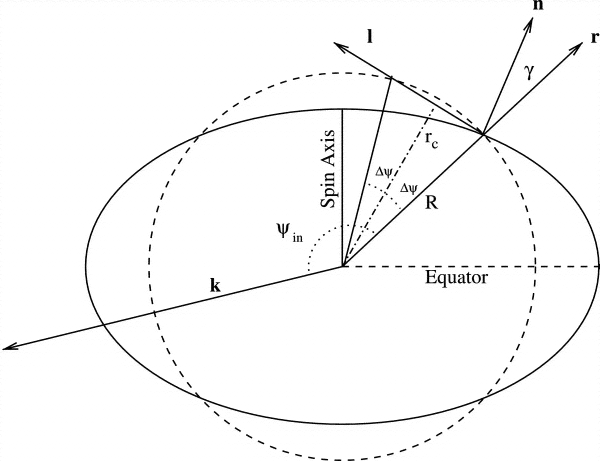
\epsfig{file=oblate_fig.png,width=8.0cm}}
\caption{Geometry of the problem. Dotted curve shows a spherical star which radius is equal to the radius of the oblate star at spot location.%Dotted curve shows the
%photon trajectory.
\label{fig:geom2}}
\end{figure}
%%%%%%%%%%%%%%%%%%%%%%%%%%%%%%%%%%%%%%%%%%%%%



We will  start the waveform with the center of the spot in the plane defined 
by the spin axis and the direction to the observer 
(when the spot crosses the plane defined by $\bmath{k}$ and $\bmath{z}$). The light pulse originating at this moment at the point that is directly below the observer and with a reference distance to the center of the star (e.g. the equator radius of the star) is used to define the zero of the observer's time coordinate. The time is zero when this photon arrives at the observer. 



We denote the unit vector along the line of sight by 
\be
\bmath{k}=(\sin i, 0, \cos i), 
\ee 
where $i$ is the inclination angle of the spin axis to the line of sight. 
Thus 
\be \label{eq:psi2}
  \cos\psi=\bmath{k}\cdot \bmath{r} = \cos i\ \cos\theta+\sin i\ \sin \theta\ \cos\phi,
\ee
Angle $\psi$ measures the apparent inclination of the spot to the line of
sight, which is different from the true inclination because of
the light bending effect.
% The initial angle of the emitted photon with respect to the normal
% ${\mathbf n}$ differs from $\psi$ because of the light bending.
We denote the initial direction of the emitted photon by $\bmath{k}_0$ ($\bmath{l}$ in figure \ref{fig:geom2})
and the true emission angle (relative to the radius vector) by $\alpha$, so that
\be
 \cos\alpha=\bmath{k}_0 \cdot \bmath{r}.
\ee
The zenith angle $\sigma$ between the $\bmath{n}$ and $\bmath{k_{0}}$ is defined by 
\be
\cos\sigma = \bmath{k_{0}}\cdot\bmath{n}.
\ee
As a photon propagates to infinity, its direction changes from
$\bmath{k}_0$ near the stellar surface to $\bmath{k}$ at infinity,
so that $\cos\alpha=\bmath{k}_0\cdot\bmath{r}$
changes to $\cos\psi=\bmath{k}\cdot\bmath{r}$.
The relation between $\bmath{k}_0$ and $\bmath{k}$ may be written as
\be\label{eq:k02}
\bmath{k}_0=[ \sin\alpha\ \bmath{k} +\sin(\psi-\alpha)\ \bmath{r}]/\sin\psi.
\ee
At any moment of time, we can introduce an instantaneous non-rotating frame $x,y,z$ 
with the $y$-axis along the direction of the spot motion, 
$x$-axis along the meridian towards the equator, and 
$z$-axis along the normal  to the spot.
In this static frame 
\be 
\bmath{k}_0=
\left( 
%\frac{\sin\alpha}{\sin\psi} (\sin i\cos\theta\cos\phi -\cos i \sin\theta),
\cos \epsilon,
\cos\xi, 
\cos\sigma
\right) ,
\ee 
where $\xi$ is the angle  between the spot velocity and $\bmath{k}_0$ :   
\be \label{eq:cosxi22}
\cos\xi=\frac{\bmath{\beta}}{\beta} \cdot \bmath{k}_0
=\frac{\sin\alpha}{\sin\psi} \frac{\bmath{\beta}}{\beta} \cdot \bmath{k}=
- \frac{\sin\alpha}{\sin\psi}\sin i\ \sin\phi\ ,
\ee
since $\bmath{\beta} = \beta(-\sin\phi,\cos\phi,0)$ in lab frame. And $\epsilon$ is the angle between the meridian 
\be
 \bmath{m} = (\cos(\theta - \gamma)\cos \phi ,\cos (\theta -\gamma)\sin \phi, -\sin (\theta -\gamma))
\ee
and $\bmath{k}_0$: 

\be \label{eq:kx-comp}
\begin{split}
\cos\epsilon= \bmath{m} \cdot \bmath{k}_0
=\frac{\sin\alpha}{\sin\psi} (\sin i \cos(\theta -\gamma)\cos \phi -\cos i \sin (\theta -\gamma)) \\ + \frac{\sin (\psi - \alpha)}{\sin \psi}(\sin \theta \cos (\theta -\gamma)-\sin (\theta -\gamma)\cos \theta).
\end{split}
\ee

%But also $\bmath{\beta}$ (y-axis) and $\bmath{n}$ (z-axis)should be perpendicular???? Okey, I think it is both same time .. +if you choose $\bmath{r}$ as z-axis, then the z-component of $\bmath{k_{0}}$ will be $\cos\alpha$)

Emission angle in the corotating frame relative to the surface normal is denoted by
$\sigma'$.  It differs from $\sigma$ because of relativistic aberration. The rays of light are tilted towards the direction of the spot motion relative to the observer.
In the frame comoving with the spot 
(with $y$-axis along the spot motion, $z$-axis along the local normal), 
the unit vector along the photon momentum  is 
obtained from the Lorentz transformation: 
\be \label{eq:k0prime2}
\bmath{k}'_0 = \Dop
\left( \begin{array}{c}
%(\sin i\cos\theta\cos\phi -\cos i \sin\theta)\sin\alpha/\sin\psi \\
\cos \epsilon \\
\Gamma (\cos\xi-\beta)\\ 
\cos\sigma
\end{array}
\right) ,
\ee 
where  the Doppler factor 
\be \label{eq:dop2}
\Dop=\frac{1}{\Gamma(1-\beta\cos\xi)} .
\ee
Using equation (\ref{eq:k0prime2}), we obtain
\be \label{eq:aberr2}
\cos\sigma' =   \Dop \ \cos\sigma ,
\ee
 
Making use of equation (\ref{eq:k02}) the zenith angle has the value
\be\label{eq:cossigma2}
\begin{split}
\cos\sigma = \bmath{k_{0}}\cdot\bmath{n} = \cos\alpha\cos\gamma+\sin\alpha\sin\gamma\cos\delta = \\
\cos \alpha  \cos \gamma + (\sin \alpha / \sin \psi) \sin \gamma (\cos i \sin \theta - \sin i \cos \theta \cos \phi),
\end{split}
\ee
where the spherical trigonometric identity $\cos i = \cos\theta\cos\psi+\sin\theta\sin\psi\cos\delta$ (where $\delta$ is the angle between spot-observer and spot-spin-axis planes) and the equation (\ref{eq:psi2}) are used. With small bending angles the approximation $\sin \alpha / \sin \psi \approx \sqrt{(1-u)}$ is used.
%if $\sin\psi\sin\theta \ne 0$. If $\sin\psi\sin\theta = 0$, then $\cos\sigma = \cos\alpha\cos\gamma$.



\subsubsection{Light bending}

The exact relation between $\alpha$ and $\psi$ (when $\alpha < \pi/2$) in Schwarzschild geometry
(i.e. light bending) is given by (...) %\citep[e.g.][]{mtw73}
\be \label{eq:bend2}
  \psi_{p}(R,\alpha)=\int_R^{\infty} \frac{dr}{r^2} \left[ \frac{1}{b^2} -
       \frac{1}{r^2}\left( 1- \frac{\rg}{r}\right)\right]^{-1/2} ,
\ee
where $b$ is impact parameter,
\be \label{eq:impact2}
  b=\frac{R}{\sqrt{1-u}} \sin\alpha .
\ee
The maximum bending angle corresponds to $\sigma=\pi/2$. Otherwise the photon would be directed across the star surface. 
The visibility of the spot is thus defined by a condition $\cos \sigma>0$. In addition one should also check that the photon won't hit the surface of the star in any later phase of it's trajectory (it might be possible for an oblate star). This check is not yet included in the current pulse profile code.

The relation between  $\alpha$ and $\psi$, when $\alpha > \pi/2$, is 
\be 
\psi(R,\alpha)=2\psi_{\max}-\psi_{p}(R,\pi-\alpha),
\ee 
where $\psi_{\max} = \psi_{p}(p,\alpha=\pi/2)$ and p is the distance of closest approach, given by
\be
p = -\frac{2}{\sqrt{3}}b\cos([arcos(3\sqrt{3}r_{s}/(2b))+2\pi]/3).
\ee




\subsubsection{Observed flux}


The observed flux from the spot 
at photon energy $E$ is
\be
\label{eq:dF_E2}
  \d F_E=I_E\ \d\Omega,
\ee
where $I_E$ is the specific   intensity of radiation
at infinity and $\d\Omega$ is
the solid angle occupied by spot with area $\d S'$ on the observer's sky.
The solid angle can be expressed in terms of the impact parameter
\be
\d\Omega=b\ \d b\ \d\varphi/D^2,
\ee
where $D$ is the distance to the source and $\varphi$ is the azimuthal
angle corresponding to rotation around line of sight (vector $\bmath{k}$).
The impact parameter $b$ depends on $\psi$ only, but not on $\varphi$.

The apparent area of the spot as measured by photon beams
in the non-rotating frame near the stellar surface is $\d S=\Dop\ \d S'$
(see Terrell 1959; Lightman et al. 1975; Ghisellini 1999) 
and the relation between $\sigma$ and $\sigma'$ is described 
by the relativistic aberration formula (for motions parallel to the 
spot surface) (\ref{eq:aberr2}). Thus the spot area projected on to the plane perpendicular 
to the photon propagation direction, i.e. a photon beam cross-section,
is Lorentz invariant (see e.g.  Lightman et al. 1975; 
Lind \& Blandford 1985): 
\be \label{eq:Salpha2}
\d S\ \cos\sigma = \d S'\ \cos\sigma' . 
\ee
%Using equation~(\ref{eq:impact2}) and
%the facts that $\d S=R^2\ \d\cos\psi\  \d\varphi$  (THIS IS NOT CORRECT %NOW) one gets... (see Morsink)
Combining this information to equation derived by (...)%\citet{MLCB07}
 the solid angle is 
\be\label{eq:omega2}
 \d\Omega=\frac{\d S' \cos \sigma'}{D^2} \frac{1}{1-u} \frac{\d\cos\alpha}{\d\cos\psi}.
\ee
In the limit of weak gravity $u\ll 1$, this gives
the usual formula $\d\Omega=\d S' \cos \sigma'/D^2$.

The combined effect of the gravitational redshift and Doppler effect
results in the following  relation between the monochromatic
observed and local intensities
(...)%\citep[see e.g.][]{mtw73,rl79}:
\be
I_{E} = \left (\frac{E}{E'}\right )^3 I'_{E '} (\sigma')
\ee
where $E/E'=\Dop \sqrt{1-u}$.
Here $I'_{E'}(\sigma')$ is the intensity computed in the frame comoving with
the spot.
For the bolometric intensity, one gets
\be
I= \left (\Dop \sqrt{1-u} \right )^4 I'(\sigma') .
\ee

The observed spectral flux (eq.~\ref{eq:dF_E2}) now reads
\be \label{eq:fluxspot2}
F_{E}=(1-u)^{1/2} \Dop^{4} I'_{E'}(\sigma') \cos\sigma
\frac{\d \cos\alpha}{\d\cos\psi}
 \frac{\d S'}{D^2} ,
\ee
where we have used the aberration formula (\ref{eq:aberr2}).
The bolometric flux is given by:
\be  \label{eq:fluxbolo2}
F= (1-u)\ \Dop^5 \
I'(\sigma')  \cos\sigma \frac{\d\cos\alpha}{\d\cos\psi} \frac{\d S'}{D^2} .
\ee
If the radiation spectrum can be represented by
a power-law $I'_{E'}(\sigma') \propto E '^{-(\Gamma-1)}$
with a photon spectral index
$\Gamma$ which does not depend on the angle $\sigma'$ then
\be \label{eq:int_trans2}
I'_{E'}(\sigma') = I'_{E}(\sigma')
\left( \Dop \sqrt{1-u} \right)^{\Gamma-1} .
\ee
The observed spectral flux at a distance $D$ from the star is then given by 
\be\label{eq:fluxplaw2}
 F_{E}= (1-u)^{\Gamma/2}\ \Dop^{\Gamma+3} I'_E(\sigma')
\cos\sigma\ \frac{\d\cos\alpha}{\d\cos\psi}\ \frac{\d S'}{D^2}.
\ee
Expression for the bolometric flux (\ref{eq:fluxbolo2})
may be obtained as a special case of Eq.~(\ref{eq:fluxplaw2}) by setting $\Gamma=2$. 

Thus, the bolometric flux from a rapidly rotating star differs by a factor  $\Dop^5$
from that for a slowly rotating star. Two powers of $\Dop$ come
from the solid angle transformation, one from the energy, one from the
photon arrival time contraction,
and the fifth from the change in the projected  area due to  aberration.
Aberration may also change the specific intensity since it has to be computed
for angle $\sigma'$ in the comoving frame




\subsubsection{Time delays}



Expressions (\ref{eq:fluxspot2}), (\ref{eq:fluxbolo2}) and (\ref{eq:fluxplaw2}) 
contain the pulsar phase $\phi$, but the flux actually corresponds to a different 
observed phase $\phiobs$, which is different from $\phi$ due to light travel delays.  
The delays become significant only for rapidly rotating pulsars.
In Schwarzschild metric the maximum time delay for a neutron star
of $M=1.4\msun$ is $\Delta t\sim 7\times 10^{-2}$ ms (almost independent
of compactness of the star $M/R$). This gives at most 
a 5 per cent correction to the arrival phase for a rotational period $P=1.5$~ms.
   
The delay is caused by different travel times of emitted
photons to the observer, depending on the position of the emitting spot.
A photon following the trajectory with an impact parameter $b$ (and $\alpha < \pi/2$)
is lagging the photon originating from a reference radius $r_{ref}$ (which can be chosen arbitrarily as long as it exceeds $\rg$) with $b=0$ by (...)%\citep{pfc83}:
:

\be \label{eq:delay2}
c\Delta t_{p}(R,\alpha)=  c\Delta t_{s}(R,\alpha) -\delta t(r_{ref},R),
\ee
where 
\be
c\Delta t_{s}(R,\alpha) =
\int_R^{\infty} \frac{\d r}{1- \rg/r}
\left\{ \left[ 1-  \frac{b^2}{r^2}  \left( 1- \frac{\rg}{r} \right)
\right] ^{-1/2}  -1 \right\}
\ee
is the time difference between photons originating from the same radius (R) and
\be
\delta t(r_{ref},R) = R-r_{ref}+\rg\ln(\frac{R-\rg}{r_{ref}-\rg})
\ee
is the time difference between photons with $b=0$ from $R$ and $r_{ref}$. 

In the case when $\alpha > \pi/2$ the corresponding delay is
\be\label{eq:delay22}
\begin{split}
c\Delta t(R,\alpha)= 2c\Delta t_{s}(p,\pi/2)-c\Delta t_{s}(R,\pi-\alpha)\\+2\left[ R-p+\rg\ln(\frac{R-\rg}{p-\rg})\right]-\delta t(r_{ref},R).
\end{split}
\ee

\iffalse
\be \label{eq:delay2}
\begin{split}
c\Delta t_{p}(R,\alpha)=  \int_R^{\infty} \frac{\d r}{1- \rg/r}
\left\{ \left[ 1-  \frac{b^2}{r^2}  \left( 1- \frac{\rg}{r} \right)
\right] ^{-1/2}  -1 \right\} \\ +\delta t(r_{ref},R),
\end{split}
\ee
where 
\be
\delta t(r_{ref},R) = R-r_{ref}+\rg\ln(\frac{R-\rg}{r_{ref}-\rg})
\ee
is the time difference between photons $b=0$ from $R$ and $r_{ref}$. 

In the case when $\alpha > \pi/2$ the corresponding delay is
\be\label{eq:delay22}
\begin{split}
c\Delta t(R,\alpha)= 2c\Delta t_{p}(p,\pi/2)-c\Delta t_{p}(R,\pi-\alpha)\\+4\left[ R-p+\rg\ln(\frac{R-\rg}{p-\rg})\right].
\end{split}
\ee

\fi

For a given pulsar phase $\phi$, we compute angle $\psi$, then
we find the corresponding emitted $\alpha$, $\sigma$ and the impact parameter
using  formulae (\ref{eq:bend2}), (\ref{eq:impact2}) and (\ref{eq:cossigma2}), and
  compute the corresponding  delays $\Delta t(R,\alpha)$ or $\Delta t_{p}(R,\alpha)$
with equations  (\ref{eq:delay2}) and (\ref{eq:delay22}).
We then construct a one-to-one
correspondence between the pulsar phase $\phi$ and
the photon arrival phase to the observer $\phiobs=\phi+ \Delta\phi$,
with the phase delays
\be \label{eq:deltaphi2}
\Delta \phi(\phi) =2\pi\nu \Delta t[b(\phi)] .
\ee

The flux at observed phase $\phiobs$ is
${F}_{\rm obs}(\phiobs)=F(\phiobs-\Delta\phi)$ with
phase delay  $\Delta \phi=2\pi\nu\Delta t$
computed using (\ref{eq:delay2}), (\ref{eq:delay22}) and (\ref{eq:deltaphi2}).
The effect of the photon arrival time contraction (or stretching) on
the observed flux is already accounted for by one of the Doppler factors, 
so there is no need to multiply again flux by $\delta$.



\subsubsection{Profiles from a large spot} 

For a finite size spot, obviously, integration over the spot surface is required. 
%I will not write here any formulae as they are rather trivial. 
The idea is to split the spot into a number of small sub-spots and compute the profiles 
from each sub-spot separately. One should be careful to include time delays correctly. 
(For this problem it is actually good to compute the time delays relative to the 
photons emitted from the point directly under the observer.) 
Integration over the spot surface is done using Gaussian quadrature in (cosine of) colatitude and trapezoidal rule for integration over the azimuth inside the spot. The surface element of the spot is 


\be \label{eq:surf_element}
\d S(\theta) = R^{2}(\theta) [1+f^{2}(\theta)]^{1/2} \sin \theta \d \theta \d \phi ,
\ee
where the factor $[1+f^{2}(\theta)]^{1/2}$ takes care of the oblateness of the spot surface (function $f(\theta)$ is given in equation \ref{eq:ftheta}).


Alternatively, one can use the HEALPIX representation of the spot, or any other routine. 
For a large spot (angular radius $\sim$30 deg), 
at least a few tens points in total are needed if one wants to achieve accuracy of the order of 1\%. 


\subsubsection{Comparison of the profiles}



\subsection{Bayesian inference}

The model presented in the previous section, can be used to constrain parameters of neutron stars by using Bayesian methods. We can fit observed data to the model and use Markov Chain Monte Carlo  (MCMC) methods to sample over the parameter space and find the most probable values for the parameters of the model. The data can also be synthetic (as in this Thesis) in order to test if the sampler will actually find the same values that were used when creating the data. More about the synthetic data is presented in the Results section. 

The aim of this work is to determine the most probable ("best-fit") values of the parameters in the pulse profile model, given the "observed" waveform, and the confidence regions for the values of these parameters. Probabilities are calculated using Bayes's theorem, which is presented in the next section. The standard Metropolis sampling method of the parameter space and a quite new ensemble sampler (used in this thesis) are discussed in the two following sections. 

\subsubsection{Bayesian analysis}

We are interested in the probability distributions of the parameters $\textbf{y}$ of the waveform model when the observed waveform is known. The probability is marked $p(\textbf{y}|D)$, where D is the energy- and oscillation phase-resolved waveform data (synthetic in this Thesis). According to the Bayes's theorem    this (posterior) probability distribution can be obtained from the likelihood of the data, given the parameter values:


\be \label{eq:bayes}
p(\textbf{y}|D) \propto p(D|\textbf{y})p(\textbf{y}).
\ee

In the previous equation $p(D|\textbf{y})$ is the likelihood or the probability distribution of the data given the parameters. The next factor $p(\textbf{y})$ is the prior probability distribution of the parameter values. As a first approximation we use uniform prior, which is the most uninformative prior. Later we take account the information of polarization measurements and make the priors of inclination and spot colatitude non-uniform to see how or if it is improving the fits. The constant of proportionality is the inverse of the normalization factor, but it is irrelevant when estimating the values of the parameters in a given model. 


\subsubsection{Metropolis (-Hastings?)}

The original, standard MCMC algorithm is called the Metropolis algorithm. It is a MCMC method for obtaining a sequence of random samples from a probability distribution. It generates random samples by moving in a random walk; that is some sequence $X_{1}...X_{t}$. Metropolis algorithm, like all the other MCMC sampling methods, satisfy the so called Markov property. It means that the conditional distribution of $X_{t+1}$ given all past elements is independent of all but the previous state:

 \be \label{eq:markov_prop}
P(X_{t+1} = x|X_{t}. . . X_{1}) = P(X_{t+1} = x|X_{t}).
\ee
A Markov chain is a random walk with Markov property.
 
The Metropolis algorithm works by taking an arbitrary move near the current
point. If $X_{t}$ is the sample at time t, then the new sample Y is propesed from the proposal distribution $q(Y|X_{t})$. The likelihood of this new sample is then compared to that of the previous sample. The likelihood ratio $\alpha$ between the to states is calculated with the following equation:
\be \label{eq:likely_ratio} 
\alpha = \frac{p(Y|D)q(X_{t}|Y)}{p(X_{t}|D)q(Y|X_{t})}.
\ee
The conditional probabilities given the data are calculated using the Bayes's formula (\ref{eq:bayes}). The ratio of these probabilites is multiplied with the ratio of proposal distributions (sometimes called transition kernels) so that the algorithm satisfy condition called detailed balance. It is an important property for proving the convergence of the chain. It states that a step from $X_{t}$ must have the same probability as a step from $Y$ to $X_{t}$.  The proposal density $q(X_{t}|Y)$ describes the probability of a transition from $Y$ j to $X_{t}$ in the parameter space.

The next step is to decide whether the likelihood ratio is high enough in order to accept the new step. In Metropolis(-Hastings) algorithm, we automatically accept a step, if $\alpha \ge 1$, but otherwise with a probability $\alpha$ (if $\alpha$ is greater than a random number between 0 and 1). If the new state is accepted, we repeat the first steps using now $Y$ as the current point. Otherwise we propose the new sample using again the same $X_{t}$. 


%If the probability distribution function (PDF) has greater value at that point, then the walk always moves there. If the PDF has a smaller value, then the move is accepted with probability dependent on how much less likely.

It can be seen that the acceptance rule simplifies considerable when the
proposal density is indeed symmetric ($q(X_{t}|Y)$=$q(Y|X_{t})$). The algorithm is typically repeated until the obtained chains are long enough in the sense that their statistics do not change significantly when adding new members to the chain. Whether the obtained samples are statistically representative of the posterior can be verified if several chains with different initial states result in the same posterior density.

Metropolis algorithm has also some limitations. The generated samples are not indpendent, since they are generated in a chain (concerns also other MCMC methods). The correlation between the samples can be measured by the autocorrelation time (ADD DEFINITION...and more). 


One major disadvantage is that the Metropolis algorithm may work poorly for skewed, or anisotropic, distributions, depending on the proposal distribution (ADD EXAMPLES). Partially for this reason we have moved to use the ensemble sampler, which is presented in the next section. 



\subsubsection{Ensemble sampler}

In this algorithm, we use a group or ensemble of sequences. Each member of
the ensemble is called a walker.

\subsubsection{Implementation}

\section{Results}

\subsection{Synthetic data}

\subsection{Parameter constraints}

\section{Summary and Conclusions}










\iffalse
%esimerkki kuvan liittämisestä
\begin{figure}
\begin{center}
\setlength{\unitlength}{1cm}
\begin{picture}(6,6)(-3,-3)
\put(-1.5,0){\vector(1,0){3}}
\put(2.7,-0.1){$\chi$}
\put(0,-1.5){\vector(0,1){3}}
\multiput(-2.5,1)(0.4,0){13}
{\line(1,0){0.2}}
\multiput(-2.5,-1)(0.4,0){13}
{\line(1,0){0.2}}
\put(0.2,1.4)
{$\beta=v/c=\tanh\chi$}
\qbezier(0,0)(0.8853,0.8853)
(2,0.9640)
\qbezier(0,0)(-0.8853,-0.8853)
(-2,-0.9640)
%\put(-3,-2){\circle*{0.2}}
\end{picture}
%\includegraphics[width=10cm]{kuva.eps}
\caption{Tässä on hieno kuva}
\label{kuva1}
\end{center}
\end{figure}
\fi


\newpage
% Rivinväli pienemmäksi viiteluettelossa. Fonttia on vaihdettava, jotta käsky
% toimisi !
\renewcommand{\baselinestretch}{1}\large\normalsize
%
\begin{thebibliography}{50}% Viiteluettelo. TÄTÄ ON PAKKO KÄYTTÄÄ !
% Jaa, ai miksi ? No, koska tällä tavalla se on vaan niin pirusti
% helpompaa.
\bibitem{lshort} T. Oetiker, H. Partl, I. Hyna and E. Schlegl,
Not so short introduction to \LaTeX 2e, 1998
\end{thebibliography}
%
% Vaihtoehtoisesti thebibliography ympäristölle voi käyttää BibTeX
% tietokantaa, jonka voit luoda tai käyttää olemassaolevaa (esim.
% Wihurilla). Suosittelemme tätä lämpimästi!
%
% Bibtex-tietokannan saa helposti tehtyä esim TeXMakerilla. Sitten
% vaan ajetaan latex gradu, bibtex gradu, latex gradu ja latex
% gradu. Ja TADAA viitteet ovat oikeassa järjestyksessä.
%
%\bibliography{/var/bib/yhdistetty}
%\bibliographystyle{wihuri}
%
\end{document} % Se oli siinä !
